%\VignetteIndexEntry{Heavy-Tailed Innovations in the R Package stochvol}
%\VignetteKeyword{Student's t distribution}
%\VignetteKeyword{data augmentation}
%\VignetteKeyword{EUR/CHF exrange rates}

\documentclass[article, nojss]{jss}

\usepackage{amsmath, amssymb}
\usepackage{bm}

\interfootnotelinepenalty=10000

\author{Gregor Kastner\\WU Vienna University of Economics and Business\\[1em]First version, May 15, 2015}
\title{Heavy-Tailed Innovations in the \proglang{R} Package \pkg{stochvol}}

%% for pretty printing and a nice hypersummary also set:
\Plainauthor{Gregor Kastner} %% comma-separated
\Plaintitle{Heavy-Tailed Innovations in the R Package stochvol} %% without formatting

%% an abstract and keywords
\Abstract{We document how sampling from a conditional Student's $t$ distribution is implemented in \pkg{stochvol}. Moreover, a simple example using EUR/CHF exchange rates illustrates how to use the augmented sampler. We conclude with results and implications.}
\Keywords{Student's $t$ distribution, data augmentation, EUR/CHF exchange rates}

%% The address of (at least) one author should be given
%% in the following format:
\Address{
  Gregor Kastner\\
  Institute for Statistics and Mathematics\\
  Department of Finance, Accounting and Statistics\\
  WU Vienna University of Economics and Business\\
  Welthandelsplatz 1, Building D4, Level 4\\
  1020 Vienna, Austria\\
  E-mail: \email{gregor.kastner@wu.ac.at}\\
  URL: \url{http://www.wu.ac.at/statmath/en/faculty_staff/faculty/gkastner/}
}

\newcommand{\mupar}{\mu}
\newcommand{\phipar}{\phi}
\newcommand{\sigmapar}{{\sigma_\eta}}
\newcommand{\sigmapartwo}{{\sigma_\eta^2}}
\newcommand{\sigmaparextrasub}[1]{\sigma_{\eta,{#1}}}
\newcommand{\allpara}{\bm{\theta}}
\newcommand{\etat}{\eta}
\newcommand{\error}{\epsilon}
\newcommand{\hsv}{h}
\newcommand{\hsvm}{\hb}
\newcommand{\y}{y}
\newcommand{\unobs}{\bm{\kappa}}
\newcommand{\sigmaeps}{{\sigma_\epsilon}}
\newcommand{\sigmaepsextrasub}[1]{\sigma_{\epsilon,{#1}}}
\newcommand{\sigmaepsextrasuper}[1]{\sigma^{#1}_\epsilon}
\newcommand{\ML}{M\!L}
\newcommand{\PL}{P\!L}
\newcommand{\CLPBF}{C\!L\!P\!B\!F}

\newcommand{\Xb}{\bm{X}}
\newcommand{\yb}{\bm{y}}
\newcommand{\betab}{\bm{\beta}}
\newcommand{\Ib}{\bm{I}}
\newcommand{\bb}[1]{\bm{b}_{#1}}
\newcommand{\Bb}[1]{\bm{B}_{#1}}
\newcommand{\bpostb}{\bm{b}_T}
\newcommand{\Bpostb}{\bm{B}_T}
\newcommand{\Sigmab}{\bm{\Sigma}}
\newcommand{\hb}{\bm{h}}
\newcommand{\pb}{\bm{p}}

\newcommand{\XtX}{\Xb^\top \Xb}

\newcommand{\Normal}[1]{\mathcal{N}\!\left(#1\right)}
\newcommand{\Normult}[2]{\mathcal{N}_{#1}\left(#2\right)}
\newcommand{\Gammainv}[1]{\mathcal{G}^{-1}\!\left(#1\right)}
\newcommand{\diag}[1]{\text{diag}({#1})}
\newcommand{\Betafun}[1]{B (#1)}
\newcommand{\Betadis}[1]{\mathcal{B}\left(#1\right)}
\newcommand{\Gammad}[1]{ \mathcal{G}\left(#1\right)}

%\DeclareMathOperator{\e}{e}
\newcommand{\e}{e}
\newcommand{\dif}{\mathrm{d}}

\newtheorem{alg}{Algorithm}

\graphicspath{{extrafig/}}
%% need no \usepackage{Sweave.sty}

\begin{document}


\section*{Preface}
This note serves as a preliminary add-on to the more elaborate article ``Dealing with Stochastic Volatility in Time Series using the \proglang{R} package \pkg{stochvol}'' \citep{kas:dea}. It discusses and relaxes the restriction to conditionally normal errors in the vanilla stochastic volatility (SV) model.

\section{The SV model with Student's $t$ errors}

Several authors have suggested to use non-normal conditional innovation distributions for stochastic volatility modeling. Examples include the Student's $t$ distribution \citep{har-etal:mul}, the extended Generalized Inverse Gaussian \citep{sil-etal:ext}, (semi-)parametric innovations \citep{jen-mah:bay, del-gri:bay}, or the GH skew Student's $t$ distribution \citep{nak-omo:sto}. In the following, we describe how the estimation of the SV model with Student's $t$ errors is implemented in the \proglang{R} \citep{r:r} package \pkg{stochvol} \citep{r:sto}.

Let $\yb = (y_1, y_2, \dots, y_n)^\top$ be a vector of returns with mean zero. The SV model with Student's $t$ errors (in short SV-$t$) is given through
\begin{eqnarray}  
 \label{m1} y_{t}|\hsv_t,\df &\sim&  \Tdist{\df}{0,\exp \hsv_t}, \\
  \label{m2} \hsv_{t}|\hsv_{t-1},\mupar, \phipar, \sigmapar&\sim& \Normal{\mupar +  \phipar (\hsv_{t-1}- \mupar ),  \sigmapartwo},\\% \etat_{t},% \qquad  \etat_{t} \sim \Normal{0,1},
 \label{m3} \hsv_0|\mu,\phi,\sigmapar &\sim& \Normal{\mu,\sigmapartwo/(1-\phi^2)},
\end{eqnarray}
i.e., conditionally on $\hsv_t$, the data is assumed to follow a zero-mean non-standardized Student's $t$ distribution with $\df$ degrees of freedom and variance $(\df \exp \hsv_t)/(\df-2)$ for $\df > 2$. Following \cite{chi-etal:mar}, we assume that a priori the degrees of freedom parameter $\df \sim \Uniform{a,b}$, i.e., follows a uniform distribution with support on the real interval $(a,b)$. All other prior components are chosen as in \cite{kas:dea}.


\section{Usage}
Estimating a stochastic volatility model with conditional $t$ errors via \pkg{stochvol} is very similar to estimating a model with standard Gaussian errors, differing only through specifying a non-\code{NA} argument \code{priornu}. This triggers the sampler specified in Section~\ref{sec:alg}. To provide an example, we investigate the historical daily EUR/CHF exchange rates and display these in Figure~\ref{fig:data}.

\begin{Schunk}
\begin{Sinput}
R> library(stochvol)
R> data(exrates)
R> par(mfrow = c(2, 1), mar = c(1.7, 1.7, 1.7, 0.1), mgp = c(1.6, 0.6, 0))
R> plot(exrates$date, exrates$CHF, type = 'l', main = 'Price of 1 EUR in CHF')
R> dat <- logret(exrates$CHF, demean = TRUE)
R> plot(exrates$date[-1], dat, type = 'l', main = 'Demeaned log returns')
\end{Sinput}
\end{Schunk}

\begin{figure}[!ht]
\begin{center}
 \includegraphics[width=\textwidth]{heavytails-data}
 \caption{Levels and demeaned log returns of EUR in CHF.}
 \label{fig:data}
\end{center}
\end{figure}

First, we fit a standard SV model to the data. Then, by specifying the argument \code{priornu} (a two-element vector containing the lower and upper bounds of the uniform prior for $\nu$), we can trigger the sampler allowing for heavy-tailed conditional innovations. 

\begin{Schunk}
\begin{Sinput}
R> res <- svsample(dat, priormu = c(-12, 1), priorphi = c(20, 1.1),
+    priorsigma = 0.1)
R> plot(res, showobs = FALSE)
\end{Sinput}
\end{Schunk}

\begin{Schunk}
\begin{Sinput}
R> rest <- svsample(dat, priormu = c(-12, 1), priorphi = c(20, 1.1),
+    priorsigma = 0.1, priornu = c(2, 100))
R> plot(rest, showobs = FALSE)
\end{Sinput}
\end{Schunk}

Results are displayed in Figure \ref{fig:res}, where the top panel (rows 1 to 3) corresponds to the output from the standard SV model and the bottom panel (rows 4 to 7) contains the output from the SV-$t$ model. Row~4 depicts $\exp(h_t/2)$ for $t \in \{1,\dots,n\}$; row~5 shows the time varying standard deviations given through $\sqrt{\nu/(\nu-2)}\exp(h_t/2)$ for $t \in \{1,\dots,n\}$; row~6 portrays trace plots and row~7 outlines the corresponding smoothed kernel density estimates for the four parameters $\mu$, $\phi$, $\sigma$, and $\nu$. It is worth noting that $\nu$ is estimated to lie between $6$ and $18$ with high posterior probability, indicating evidence for the presence of heavy tails even after catering for stochastic volatility. The extra flexibility of the SV-$t$ sampler seems to allow for increased persistence $\phi$ and smaller variance of log-volatility $\sigma^2$, resulting in smoother time-varying volatility estimates.

\begin{figure}[p]
\begin{center}
 \includegraphics[width=\textwidth]{heavytails-normalerr}
 \vspace{2em}

 \includegraphics[width=\textwidth]{heavytails-terr}
 \caption{Standard output of the \code{plot} method when applied to an \code{svdraws} object containing posterior draws from an SV model with Gaussian errors (top) and Student's $t$ errors (bottom).}
 \label{fig:res}
\end{center}
\end{figure}

We investigate one-day-ahead out-of-sample predictive performance of an AR(1) model with (a) homoskedastic, (b) SV, (c) SV-$t$, (d) GARCH(1,1) errors, applied to the raw exchange rate data. Details about this procedure are provided in Chapter~5 of \cite{kas:dea}. The results, summarized in Figure~\ref{fig2}, speak in favor of the SV-$t$ model for this dataset.

\begin{figure}[p]
\begin{center}
 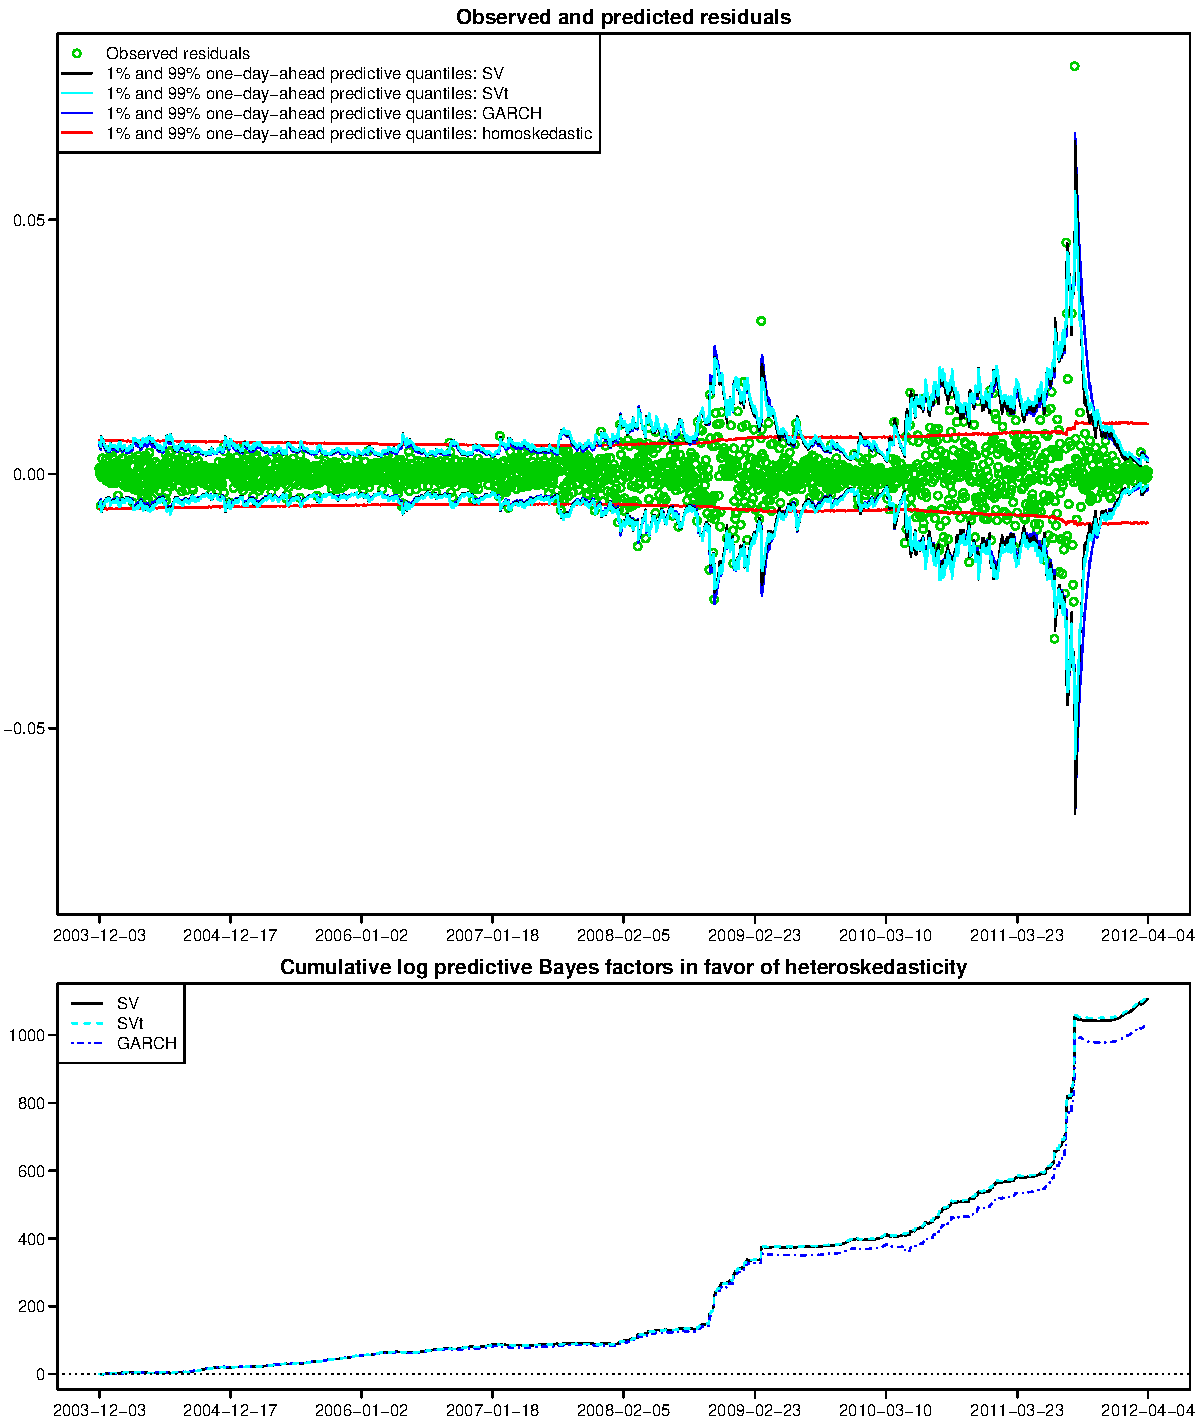
\includegraphics[width=\textwidth]{predlik_terr}
 \caption{Log predictive one-day-ahead Bayes factors in favor of SV, SV-$t$, and GARCH errors over the homoskedastic model. The final log predictive Bayes factors aggregate to 1107.44 (SV), 1115.36 (SV-$t$), and 1033.53 (GARCH), respectively, thus providing strong evidence for the SV-$t$ model.}
 \label{fig2}
\end{center}
\end{figure}

\section{Necessary modifications in the sampling scheme}
\label{sec:alg}

The Student's $t$ distribution appearing in Equation \ref{m1} can be conveniently expressed as a scale mixture of normal distributions,
\begin{eqnarray*}
y_{t}|\hsv_t,\taug_t &\sim&  \Normal{0, \taug_t \exp{\hsv_{t}}},%\error_{t},% \qquad \error_{t} \sim \Normal{0,1},
 \\
 \taug_t|\df &\sim& \Gammainv{\df/2, \df/2},
\end{eqnarray*}
where $\Normal{\mu, \sigmapartwo}$ denotes the normal distribution with mean $\mu$ and variance $\sigmapartwo$, and $\Gammainv{a,b}$ denotes the inverse gamma distribution with shape and scale parameters $a$ and $b$, respectively.

Treating $\taugm = (\taug_1, \dots, \taug_n)^\top$ as latent data and letting $\tilde y_t = y_t/\sqrt{\taug_t}$ for $t \in \{1,\dots,n\},$ we have
\[
\tilde y_t|\hsv_t \sim \Normal{0, \exp{h_t}},
\]
and the AWOL sampler described in \cite{kas-fru:anc} can directly be applied to the transformed data. To obtain draws from the newly introduced variables $\taugm$ and $\df$, two additional steps are required.

\subsection{Sampling the auxiliary variables}

It is easy to see that the marginal posterior is given through
\[
\taug_t|y_t,\hsv_t,\df \sim \Gammainv{\frac{\df + 1}{2},\frac{\df + y_t^2\exp(-\hsv_t)}{2}},
\]
independently for each $t \in \{1, \dots, n\}$. Obtaining draws from this distribution is straightforward.

\subsection{Sampling the degrees of freedom parameter}

The full conditional posterior of the degrees of freedom parameter, $\df|\cdot$, only depends on $\taugm$. Its density is given through the product of $n$ univariate truncated inverse gamma densities which may be written as
\begin{eqnarray}
 \label{dfdens}
p(\df|\cdot) = p(\df|\taugm) \propto
\left(\frac{\df}{2}\right)^{n\df/2}
\Gamma\!\left(\frac{\df}{2}\right)^{-n}
\left(\prod_{t=1}^n \taug_t\right)^{-\df/2}
\exp\left\{-\frac{\df}{2}\sum_{t=1}^n\frac{1}{\taug_t}\right\}
\end{eqnarray}
for $\df \in (a,b)$ and zero elsewhere.

For obtaining draws from this distribution, we use an independence Metropolis-Hastings update. We follow \cite{chi-gre:bay}, who introduced the idea of specifying an independence proposal through numerical maximization of the log-density. For the problem at hand, we consequently aim for optimizing
\begin{eqnarray}
 \label{logdfdens}
\log p(\df|\taugm) = \frac{n\df}{2}\log(\df/2) -
n\log\Gamma(\df/2)-
\frac{\df}{2}\sum_{t=1}^n\!\left(\log\taug_t+\frac{1}{\taug_t}\right) + C,
\end{eqnarray}
with first and second derivatives given through
\begin{eqnarray}
 \label{d1}
 \frac{\partial \log p(\df|\taugm)}{\partial \df} &=&
 \frac{n}{2}\left(1 + \log(\df/2) -\psi^{(0)}(\nu/2)\right) -
 \frac{1}{2}\sum_{t=1}^n\!\left(\log\taug_t + \frac{1}{\taug_t}\right),\\
\label{d2}
\frac{\partial^2 \log p(\df|\taugm)}{\partial \df^2} &=&
\frac{n}{2\df} - \frac{n}{4}\psi^{(1)}(\nu/2),
\end{eqnarray}
where $\psi^{(m)}$ denotes the polygamma function of order $m$. Using the above, it is easy to numerically find
\begin{eqnarray*}
\hat \df &=& \arg\max_{\df} \log p(\df|\taugm),\\
B_{\hat \df} &=& \left.-1\middle/\frac{\partial^2 \log p(\df|\taugm)}{\partial \df^2}\right|_{\df=\hat\df},
\end{eqnarray*}
and a proposal candidate $\df_\text{prop}$ may be drawn from a normal distribution with mean $\hat\df$ and variance $B_{\hat \df}$ (the Laplace approximation). Letting $\phi(x| \hat\df, B_{\hat \df})$ denote the corresponding density function, the acceptance probability is equal to $\min\{1,R\}$ with
\[
R = \frac{p(\df_\text{prop}|\taugm)}{p(\df_\text{old}|\taugm)} \times
\frac{\phi(\df_\text{old}| \hat \df, B_{\hat \df})}{\phi(\df_\text{prop}| \hat \df, B_{\hat \df})}.
\
\]

\section{Conclusion}
We have shown how a simply data augmentation trick can be utilized to generalize the core sampler in \pkg{stochvol} in order to cater for potentially heavier-tailed innovation distributions. However, several caveats are called for:
\begin{itemize}
 \item Even though the uniform prior for $\nu$ has been used widely, more robust alternatives are probably preferred, cf.\ \cite{fru-pay:bay} and the references therein.
 \item Sampling the degrees of freedom parameter $\nu$ conditionally on $\bm{\tau}$ can be very inefficient if $\nu$ becomes large (and thus the plain vanilla SV model suffices). We recommend to resort to the original SV sampler in this case.
 \item Leaving aside the additional computational burden, it is trivial to incorporate this extension into samplers employing \pkg{stochvol} as part of a larger MCMC scheme \citep[e.g.][]{hub:den, kas-etal:ana, dov-etal:doe}. Nevertheless, at the current stage of development, this should be conducted with caution by carefully investigating the convergence of the posterior draws.
\end{itemize}

\section*{Acknowledgments}
The author would like to thank the attendants of the Spring 2015 Brown Bag Seminar of the Institute for Statistics and Mathematics, WU Vienna University of Economics and Business, in particular Sylvia Fr\"{u}hwirth-Schnatter, Mark Jensen, and Kurt Hornik, for stimulating comments and suggestions.

\bibliography{mybib}


\end{document}

